\documentclass[]{article}
\usepackage{lmodern}
\usepackage{amssymb,amsmath}
\usepackage{ifxetex,ifluatex}
\usepackage{fixltx2e} % provides \textsubscript
\ifnum 0\ifxetex 1\fi\ifluatex 1\fi=0 % if pdftex
  \usepackage[T1]{fontenc}
  \usepackage[utf8]{inputenc}
\else % if luatex or xelatex
  \ifxetex
    \usepackage{mathspec}
  \else
    \usepackage{fontspec}
  \fi
  \defaultfontfeatures{Ligatures=TeX,Scale=MatchLowercase}
\fi
% use upquote if available, for straight quotes in verbatim environments
\IfFileExists{upquote.sty}{\usepackage{upquote}}{}
% use microtype if available
\IfFileExists{microtype.sty}{%
\usepackage{microtype}
\UseMicrotypeSet[protrusion]{basicmath} % disable protrusion for tt fonts
}{}
\usepackage[margin=1in]{geometry}
\usepackage{hyperref}
\hypersetup{unicode=true,
            pdftitle={Cincia de Dados para Todos (Data Science For All) - 2018.1 - Anlise da Produo Cientfica e Acadmica da Universidade de Braslia - Relatrio Final da Disciplina - \textless{}81\textgreater{}reas Geografia, Geocincias Aplicadas e Geodinmica e Geologia},
            pdfborder={0 0 0},
            breaklinks=true}
\urlstyle{same}  % don't use monospace font for urls
\usepackage{color}
\usepackage{fancyvrb}
\newcommand{\VerbBar}{|}
\newcommand{\VERB}{\Verb[commandchars=\\\{\}]}
\DefineVerbatimEnvironment{Highlighting}{Verbatim}{commandchars=\\\{\}}
% Add ',fontsize=\small' for more characters per line
\usepackage{framed}
\definecolor{shadecolor}{RGB}{248,248,248}
\newenvironment{Shaded}{\begin{snugshade}}{\end{snugshade}}
\newcommand{\KeywordTok}[1]{\textcolor[rgb]{0.13,0.29,0.53}{\textbf{#1}}}
\newcommand{\DataTypeTok}[1]{\textcolor[rgb]{0.13,0.29,0.53}{#1}}
\newcommand{\DecValTok}[1]{\textcolor[rgb]{0.00,0.00,0.81}{#1}}
\newcommand{\BaseNTok}[1]{\textcolor[rgb]{0.00,0.00,0.81}{#1}}
\newcommand{\FloatTok}[1]{\textcolor[rgb]{0.00,0.00,0.81}{#1}}
\newcommand{\ConstantTok}[1]{\textcolor[rgb]{0.00,0.00,0.00}{#1}}
\newcommand{\CharTok}[1]{\textcolor[rgb]{0.31,0.60,0.02}{#1}}
\newcommand{\SpecialCharTok}[1]{\textcolor[rgb]{0.00,0.00,0.00}{#1}}
\newcommand{\StringTok}[1]{\textcolor[rgb]{0.31,0.60,0.02}{#1}}
\newcommand{\VerbatimStringTok}[1]{\textcolor[rgb]{0.31,0.60,0.02}{#1}}
\newcommand{\SpecialStringTok}[1]{\textcolor[rgb]{0.31,0.60,0.02}{#1}}
\newcommand{\ImportTok}[1]{#1}
\newcommand{\CommentTok}[1]{\textcolor[rgb]{0.56,0.35,0.01}{\textit{#1}}}
\newcommand{\DocumentationTok}[1]{\textcolor[rgb]{0.56,0.35,0.01}{\textbf{\textit{#1}}}}
\newcommand{\AnnotationTok}[1]{\textcolor[rgb]{0.56,0.35,0.01}{\textbf{\textit{#1}}}}
\newcommand{\CommentVarTok}[1]{\textcolor[rgb]{0.56,0.35,0.01}{\textbf{\textit{#1}}}}
\newcommand{\OtherTok}[1]{\textcolor[rgb]{0.56,0.35,0.01}{#1}}
\newcommand{\FunctionTok}[1]{\textcolor[rgb]{0.00,0.00,0.00}{#1}}
\newcommand{\VariableTok}[1]{\textcolor[rgb]{0.00,0.00,0.00}{#1}}
\newcommand{\ControlFlowTok}[1]{\textcolor[rgb]{0.13,0.29,0.53}{\textbf{#1}}}
\newcommand{\OperatorTok}[1]{\textcolor[rgb]{0.81,0.36,0.00}{\textbf{#1}}}
\newcommand{\BuiltInTok}[1]{#1}
\newcommand{\ExtensionTok}[1]{#1}
\newcommand{\PreprocessorTok}[1]{\textcolor[rgb]{0.56,0.35,0.01}{\textit{#1}}}
\newcommand{\AttributeTok}[1]{\textcolor[rgb]{0.77,0.63,0.00}{#1}}
\newcommand{\RegionMarkerTok}[1]{#1}
\newcommand{\InformationTok}[1]{\textcolor[rgb]{0.56,0.35,0.01}{\textbf{\textit{#1}}}}
\newcommand{\WarningTok}[1]{\textcolor[rgb]{0.56,0.35,0.01}{\textbf{\textit{#1}}}}
\newcommand{\AlertTok}[1]{\textcolor[rgb]{0.94,0.16,0.16}{#1}}
\newcommand{\ErrorTok}[1]{\textcolor[rgb]{0.64,0.00,0.00}{\textbf{#1}}}
\newcommand{\NormalTok}[1]{#1}
\usepackage{longtable,booktabs}
\usepackage{graphicx,grffile}
\makeatletter
\def\maxwidth{\ifdim\Gin@nat@width>\linewidth\linewidth\else\Gin@nat@width\fi}
\def\maxheight{\ifdim\Gin@nat@height>\textheight\textheight\else\Gin@nat@height\fi}
\makeatother
% Scale images if necessary, so that they will not overflow the page
% margins by default, and it is still possible to overwrite the defaults
% using explicit options in \includegraphics[width, height, ...]{}
\setkeys{Gin}{width=\maxwidth,height=\maxheight,keepaspectratio}
\IfFileExists{parskip.sty}{%
\usepackage{parskip}
}{% else
\setlength{\parindent}{0pt}
\setlength{\parskip}{6pt plus 2pt minus 1pt}
}
\setlength{\emergencystretch}{3em}  % prevent overfull lines
\providecommand{\tightlist}{%
  \setlength{\itemsep}{0pt}\setlength{\parskip}{0pt}}
\setcounter{secnumdepth}{0}
% Redefines (sub)paragraphs to behave more like sections
\ifx\paragraph\undefined\else
\let\oldparagraph\paragraph
\renewcommand{\paragraph}[1]{\oldparagraph{#1}\mbox{}}
\fi
\ifx\subparagraph\undefined\else
\let\oldsubparagraph\subparagraph
\renewcommand{\subparagraph}[1]{\oldsubparagraph{#1}\mbox{}}
\fi

%%% Use protect on footnotes to avoid problems with footnotes in titles
\let\rmarkdownfootnote\footnote%
\def\footnote{\protect\rmarkdownfootnote}

%%% Change title format to be more compact
\usepackage{titling}

% Create subtitle command for use in maketitle
\newcommand{\subtitle}[1]{
  \posttitle{
    \begin{center}\large#1\end{center}
    }
}

\setlength{\droptitle}{-2em}
  \title{Cincia de Dados para Todos (Data Science For All) - 2018.1 - Anlise da
Produo Cientfica e Acadmica da Universidade de Braslia - Relatrio Final
da Disciplina - \textless{}81\textgreater{}reas Geografia, Geocincias
Aplicadas e Geodinmica e Geologia}
  \pretitle{\vspace{\droptitle}\centering\huge}
  \posttitle{\par}
  \author{}
  \preauthor{}\postauthor{}
  \predate{\centering\large\emph}
  \postdate{\par}
  \date{02/07/2018}


\begin{document}
\maketitle

\section{Introdu????o}\label{introduo}

\section{Metodologia}\label{metodologia}

A metodologia aplicada para produ????o desse relat??rio ?? a \emph{Cross
Industry Standard Process for Data Mining} (CRISP-DM). O CRISP-DM divide
o processo de minera????o de dados em seis fases principais. A
sequ??ncia dessas fases n??o ?? rigorosa e se move iterativamente entre
as fases, como for necess??rio.

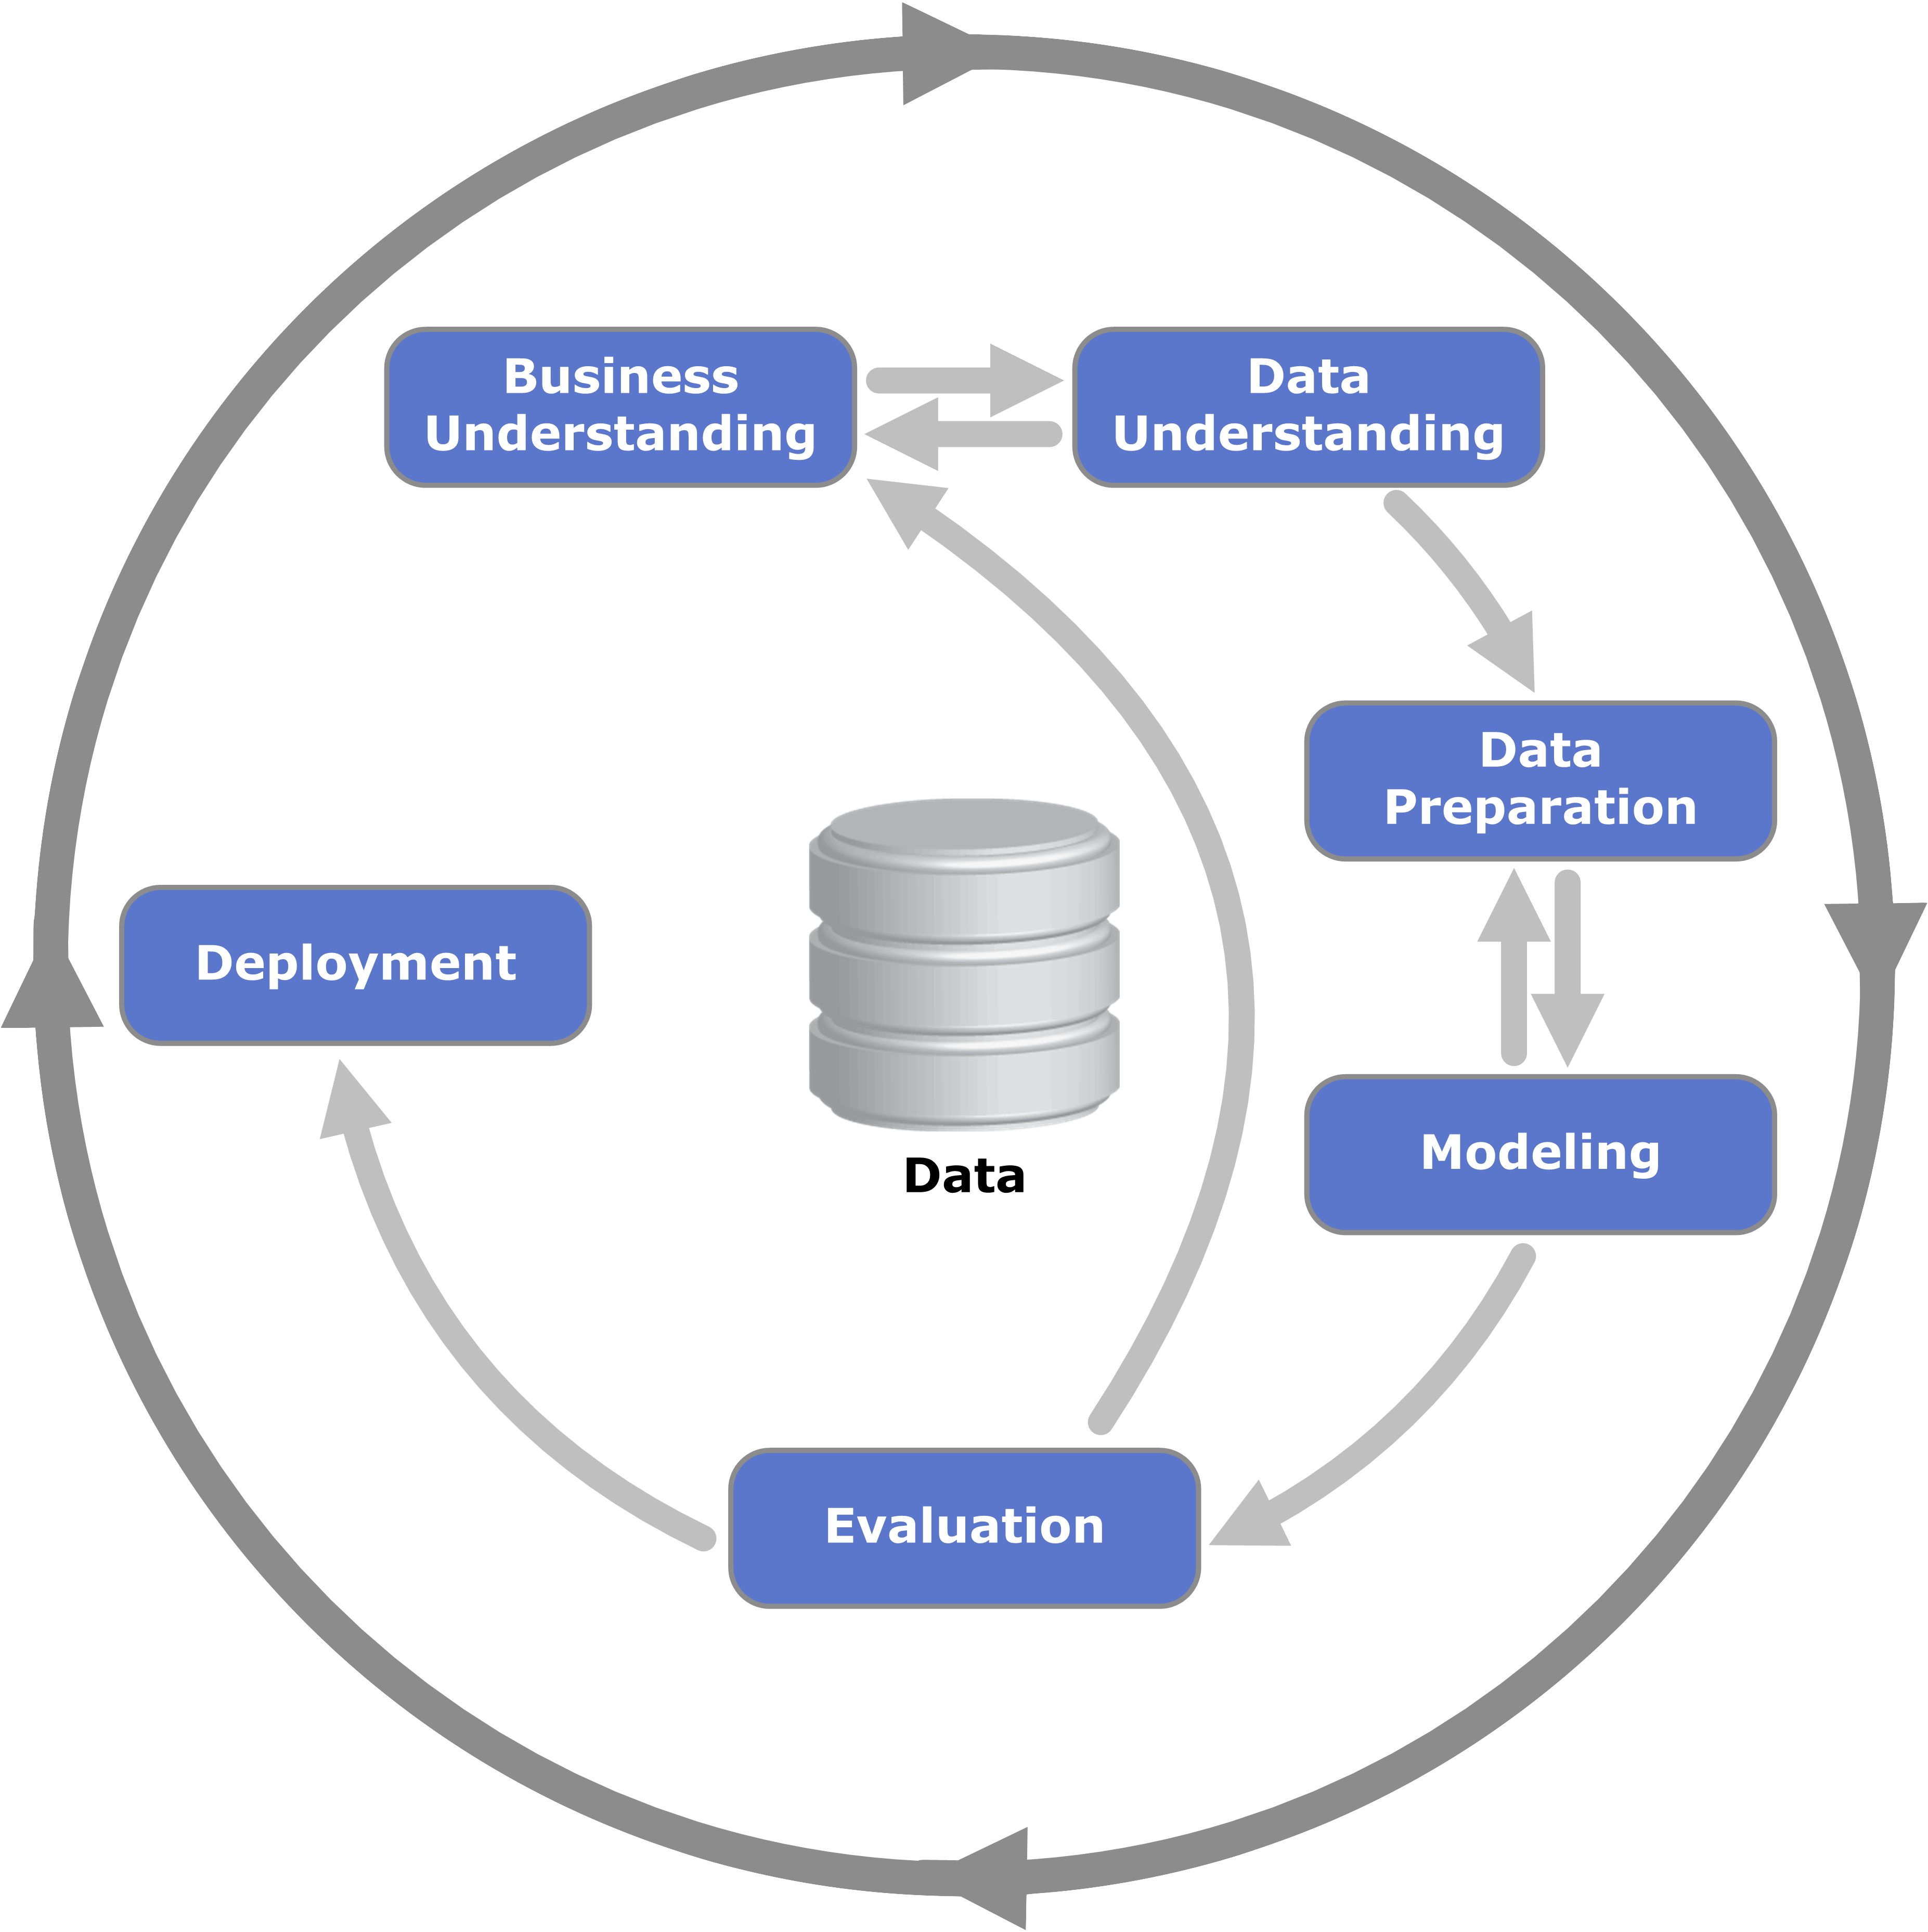
\includegraphics{images/CRISP-DM_Process_Diagram.png} \emph{Figura I}

Na \emph{figura I} as setas mostradas na imagem do processo indicam as
depend??ncias mais importantes e ocorrentes entre as fases do processo.
O c??rculo externo no diagrama simboliza a natureza c??clica da pr??pria
minera????o de dados. Um processo de minera????o de dados continua
depois que uma solu????o foi implementada.

\subsection{Delimita????es iniciais}\label{delimitaes-iniciais}

\subsubsection{Dom??nio de Aplica????o do
projeto}\label{domnio-de-aplicao-do-projeto}

\subsubsection{Tipo de Problema
abordado}\label{tipo-de-problema-abordado}

\subsubsection{Conjunto de Ferramentas e
T??cnicas}\label{conjunto-de-ferramentas-e-tcnicas}

\subsection{Modelo de Refer??ncia
CRISP-DM}\label{modelo-de-referncia-crisp-dm}

O ciclo de vida completo de um projeto de minera????o de dados ??
representado em seis fases, no processo do CRISP-DM. Na \emph{figura II}
?? esbo??ado as fases acompanhados das tarefas e sa??das geradas.

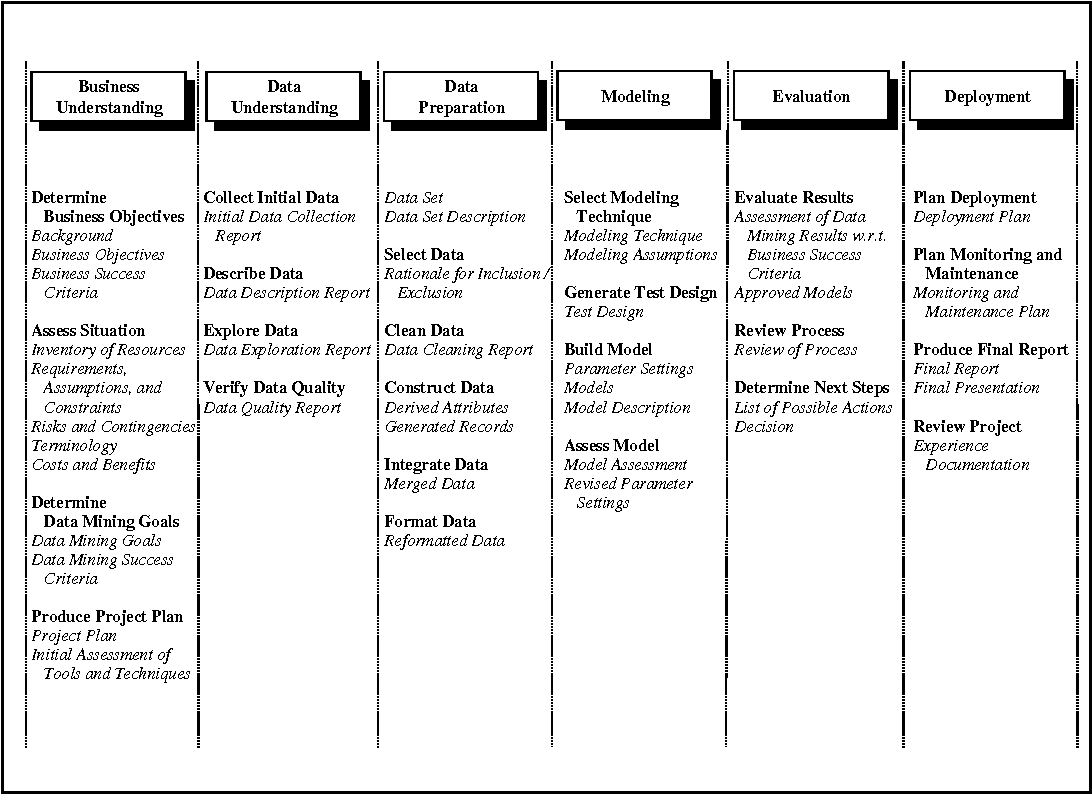
\includegraphics{images/crisp-dm-phases.png} \emph{Figura II}

\subsection{Como surgiu o CRISP-DM?}\label{como-surgiu-o-crisp-dm}

O CRISP-DM foi idealizado no ano de 1996 e se tornou um projeto da
Uni??o Europeia sob a iniciativa de financiamento \emph{European
Strategic Program on Research in Information Technology} (ESPRIT) no ano
de 1997. O projeto foi liderado por cinco empresas: SPSS, Teradata,
Daimler AG, NCR Corporation e OHRA. O modelo de trabalho nasceu a partir
da iniciativa de profissionais que trabalhavam com data mining.

\subsubsection{Por que usar o CRISP-DM?}\label{por-que-usar-o-crisp-dm}

\subsubsection{Organiza????o hier??rquica de atividades em
fases}\label{organizao-hierrquica-de-atividades-em-fases}

\subsubsection{Seis Fases do CRISP-DM}\label{seis-fases-do-crisp-dm}

\section{CRISP-DM Fase 1 - Entendimento do
Neg??cio}\label{crisp-dm-fase-1---entendimento-do-negcio}

\subsection{O que ?? o Sistema Nacional de P??s-Gradua????o?
(Contextualiza????o)}\label{o-que-o-sistema-nacional-de-ps-graduao-contextualizao}

\subsubsection{Os Col??gios, Grandes ??reas e ??reas da P??s-Gradua????o
Brasileira}\label{os-colgios-grandes-reas-e-reas-da-ps-graduao-brasileira}

\paragraph{Col??gio de Ci??ncias da
vida}\label{colgio-de-cincias-da-vida}

\begin{longtable}[]{@{}lll@{}}
\toprule
CI??NCIAS AGR??RIAS & CI??NCIAS BIOL??GICAS & CI??NCIAS DA
SA??DE\tabularnewline
\midrule
\endhead
Ci??ncia de Alimentos & Biodiversidade & Educa????o
F??sica\tabularnewline
Ci??ncias Agr??rias I & Ci??ncias Biol??gicas I &
Enfermagem\tabularnewline
Medicina Veterin??ria & Ci??ncias Biol??gicas II &
Farm??cia\tabularnewline
Zootecnia / Recursos Pesqueiros & Ci??ncias Biol??gicas III & Medicina
I\tabularnewline
- & - & Medicina II\tabularnewline
- & - & Medicina III\tabularnewline
- & - & Nutri????o\tabularnewline
- & - & Odontologia\tabularnewline
- & - & Sa??de Coletiva\tabularnewline
\bottomrule
\end{longtable}

\paragraph{Col??gio de Ci??ncias Exatas, Tecnol??gicas e
Multidisciplinar}\label{colgio-de-cincias-exatas-tecnolgicas-e-multidisciplinar}

\begin{longtable}[]{@{}lll@{}}
\toprule
CI??NCIAS EXATAS E DA TERRA & ENGENHARIAS &
MULTIDISCIPLINAR\tabularnewline
\midrule
\endhead
Astronomia / F??sica & Engenharias I & Biotecnologia\tabularnewline
Ci??ncia da Computa????o & Engenharias II & Ci??ncias
Ambientais\tabularnewline
Geoci??ncias & Engenharias III & Ensino\tabularnewline
Matem??tica / Probabilidade e Estat??stica & Engenharias IV &
Interdisciplinar\tabularnewline
Qu??mica & - & Materiais\tabularnewline
\bottomrule
\end{longtable}

\paragraph{Col??gio de Humanidades}\label{colgio-de-humanidades}

\begin{longtable}[]{@{}lll@{}}
\toprule
\begin{minipage}[b]{0.03\columnwidth}\raggedright\strut
CI??NCIAS HUMANAS\strut
\end{minipage} & \begin{minipage}[b]{0.03\columnwidth}\raggedright\strut
CI??NCIAS SOCIAIS APLICADAS\strut
\end{minipage} & \begin{minipage}[b]{0.03\columnwidth}\raggedright\strut
LINGU??STICA, LETRAS E ARTES\strut
\end{minipage}\tabularnewline
\midrule
\endhead
\begin{minipage}[t]{0.03\columnwidth}\raggedright\strut
Antropol/Arqueol\strut
\end{minipage} & \begin{minipage}[t]{0.03\columnwidth}\raggedright\strut
Admin.P??b./Empr.,C.Cont??b. e Tur.\strut
\end{minipage} & \begin{minipage}[t]{0.03\columnwidth}\raggedright\strut
Artes\strut
\end{minipage}\tabularnewline
\begin{minipage}[t]{0.03\columnwidth}\raggedright\strut
Ci??ncia Pol. e Rel. Int.\strut
\end{minipage} & \begin{minipage}[t]{0.03\columnwidth}\raggedright\strut
Arquit., Urban. e Design\strut
\end{minipage} & \begin{minipage}[t]{0.03\columnwidth}\raggedright\strut
Lingu??stica e Literatura\strut
\end{minipage}\tabularnewline
\begin{minipage}[t]{0.03\columnwidth}\raggedright\strut
Ci??ncias da Religi??o e Teol.\strut
\end{minipage} & \begin{minipage}[t]{0.03\columnwidth}\raggedright\strut
Comunica????o e Informa????o\strut
\end{minipage} & \begin{minipage}[t]{0.03\columnwidth}\raggedright\strut
-\strut
\end{minipage}\tabularnewline
\begin{minipage}[t]{0.03\columnwidth}\raggedright\strut
Educa????o\strut
\end{minipage} & \begin{minipage}[t]{0.03\columnwidth}\raggedright\strut
Direito\strut
\end{minipage} & \begin{minipage}[t]{0.03\columnwidth}\raggedright\strut
-\strut
\end{minipage}\tabularnewline
\begin{minipage}[t]{0.03\columnwidth}\raggedright\strut
Filosofia\strut
\end{minipage} & \begin{minipage}[t]{0.03\columnwidth}\raggedright\strut
Economia\strut
\end{minipage} & \begin{minipage}[t]{0.03\columnwidth}\raggedright\strut
-\strut
\end{minipage}\tabularnewline
\begin{minipage}[t]{0.03\columnwidth}\raggedright\strut
Geografia\strut
\end{minipage} & \begin{minipage}[t]{0.03\columnwidth}\raggedright\strut
Planej. Urbano e Reg. / Demografia\strut
\end{minipage} & \begin{minipage}[t]{0.03\columnwidth}\raggedright\strut
-\strut
\end{minipage}\tabularnewline
\begin{minipage}[t]{0.03\columnwidth}\raggedright\strut
Hist??ria\strut
\end{minipage} & \begin{minipage}[t]{0.03\columnwidth}\raggedright\strut
Servi??o Social\strut
\end{minipage} & \begin{minipage}[t]{0.03\columnwidth}\raggedright\strut
-\strut
\end{minipage}\tabularnewline
\begin{minipage}[t]{0.03\columnwidth}\raggedright\strut
Psicologia\strut
\end{minipage} & \begin{minipage}[t]{0.03\columnwidth}\raggedright\strut
-\strut
\end{minipage} & \begin{minipage}[t]{0.03\columnwidth}\raggedright\strut
-\strut
\end{minipage}\tabularnewline
\begin{minipage}[t]{0.03\columnwidth}\raggedright\strut
Sociologia\strut
\end{minipage} & \begin{minipage}[t]{0.03\columnwidth}\raggedright\strut
-\strut
\end{minipage} & \begin{minipage}[t]{0.03\columnwidth}\raggedright\strut
-\strut
\end{minipage}\tabularnewline
\bottomrule
\end{longtable}

\subsection{A UnB dentro do Sistema Nacional de P??s-Gradua????o
(Contextualiza????o)}\label{a-unb-dentro-do-sistema-nacional-de-ps-graduao-contextualizao}

\subsubsection{O que ?? a UnB?}\label{o-que-a-unb}

\subsubsection{Descri????o das p??s-gradua????es da
UnB}\label{descrio-das-ps-graduaes-da-unb}

\subsubsection{Outros aspectos que caracterizam a produ????o cient??fica
e acad??mica da
UnB}\label{outros-aspectos-que-caracterizam-a-produo-cientfica-e-acadmica-da-unb}

\subsection{O que a Organiza????o precisa realmente
alcan??ar?}\label{o-que-a-organizao-precisa-realmente-alcanar}

\subsection{Avalia????o das
Circunst??ncias}\label{avaliao-das-circunstncias}

\subsubsection{Avalia????o preliminar das p??s-gradua????es na
UnB}\label{avaliao-preliminar-das-ps-graduaes-na-unb}

\subsubsection{Avalia????o preliminar da produ????o cient??fica e
acad??mica da
UnB}\label{avaliao-preliminar-da-produo-cientfica-e-acadmica-da-unb}

\section{CRISP-DM Fase 2 - Entendimento dos
Dados}\label{crisp-dm-fase-2---entendimento-dos-dados}

\subsection{CRISP-DM Fase.Atividade 2.1 - Coleta inicial dos
dados}\label{crisp-dm-fase.atividade-2.1---coleta-inicial-dos-dados}

\subsubsection{Perfil profissional dos docentes vinculados ??s
p??s-gradua????es}\label{perfil-profissional-dos-docentes-vinculados-s-ps-graduaes}

\subsubsection{Orienta????es de mestrado e doutorado realizadas pelos
docentes vinculados ??s
p??s-gradua????es}\label{orientaes-de-mestrado-e-doutorado-realizadas-pelos-docentes-vinculados-s-ps-graduaes}

\subsubsection{Produ????o bibliogr??fica gerada pelos docentes
vinculados ??s
p??s-gradua????es}\label{produo-bibliogrfica-gerada-pelos-docentes-vinculados-s-ps-graduaes}

\subsubsection{Agrupamento dos docentes conforme ??reas de
atua????o}\label{agrupamento-dos-docentes-conforme-reas-de-atuao}

\subsubsection{Redes de colabora????o entre
docentes}\label{redes-de-colaborao-entre-docentes}

\subsection{CRISP-DM Fase.Atividade 2.2 - Descri????o dos
Dados}\label{crisp-dm-fase.atividade-2.2---descrio-dos-dados}

Para leitura e manipula????o dos dados utilizados, ser??o utilizadas
primordialmente as cinco bibliotecas a seguirs

\begin{Shaded}
\begin{Highlighting}[]
\KeywordTok{library}\NormalTok{(jsonlite)}
\KeywordTok{library}\NormalTok{(listviewer)}
\KeywordTok{library}\NormalTok{(readxl)}
\KeywordTok{library}\NormalTok{(ggplot2)}
\KeywordTok{library}\NormalTok{(tidyverse)}
\end{Highlighting}
\end{Shaded}

\begin{verbatim}
## -- Attaching packages ----------------------------------------- tidyverse 1.2.1 --
\end{verbatim}

\begin{verbatim}
## <U+221A> tibble  1.4.2     <U+221A> purrr   0.2.4
## <U+221A> tidyr   0.8.0     <U+221A> dplyr   0.7.4
## <U+221A> readr   1.1.1     <U+221A> stringr 1.3.0
## <U+221A> tibble  1.4.2     <U+221A> forcats 0.3.0
\end{verbatim}

\begin{verbatim}
## -- Conflicts -------------------------------------------- tidyverse_conflicts() --
## x dplyr::filter()  masks stats::filter()
## x purrr::flatten() masks jsonlite::flatten()
## x dplyr::lag()     masks stats::lag()
\end{verbatim}

\subsubsection{Descri????o dos dados do
perfil}\label{descrio-dos-dados-do-perfil}

\paragraph{Potencial de utiliza????o dos dados do perfil dos
docentes}\label{potencial-de-utilizao-dos-dados-do-perfil-dos-docentes}

\subsubsection{Descri????o dos dados de
orienta????es}\label{descrio-dos-dados-de-orientaes}

\subsubsection{Descri????o dos dados de produ????o
bibliogr??fica}\label{descrio-dos-dados-de-produo-bibliogrfica}

\subsubsection{Descri????o dos dados de agrega????o de docentes por
??rea}\label{descrio-dos-dados-de-agregao-de-docentes-por-rea}

\subsubsection{Descri????o dos dados de redes de
colabora????o}\label{descrio-dos-dados-de-redes-de-colaborao}

\subsection{CRISP-DM Fase.Atividade 2.3 - An??lise explorat??ria dos
dados}\label{crisp-dm-fase.atividade-2.3---anlise-exploratria-dos-dados}

\subsubsection{Arquivo Profile}\label{arquivo-profile}

\subsubsection{Arquivo Publica????o}\label{arquivo-publicao}

\subsubsection{Arquivo Orienta????o}\label{arquivo-orientao}

\subsection{CRISP-DM Fase.Atividade 2.4 - Verifica????o da qualidade dos
dados.}\label{crisp-dm-fase.atividade-2.4---verificao-da-qualidade-dos-dados.}

\section{\texorpdfstring{CRISP-DM Fase 3 - \textbf{Prepara????o dos
Dados}}{CRISP-DM Fase 3 - Prepara????o dos Dados}}\label{crisp-dm-fase-3---preparao-dos-dados}

\subsection{CRISP-DM Fase.Atividade 3.1 - Sele????o dos
dados.}\label{crisp-dm-fase.atividade-3.1---seleo-dos-dados.}

\subsection{CRISP-DM Fase.Atividade 3.2 - Limpeza dos
dados}\label{crisp-dm-fase.atividade-3.2---limpeza-dos-dados}

\subsection{CRISP-DM Fase.Atividade 3.3 - Constru????o dos
dados}\label{crisp-dm-fase.atividade-3.3---construo-dos-dados}

\subsection{CRISP-DM Fase.Atividade 3.4 - Integra????o dos
dados}\label{crisp-dm-fase.atividade-3.4---integrao-dos-dados}

\subsection{CRISP-DM Fase.Atividade 3.5 - Formata????o dos
dados}\label{crisp-dm-fase.atividade-3.5---formatao-dos-dados}

\section{\texorpdfstring{CRISP-DM Fase 4 -
\textbf{Modelagem}}{CRISP-DM Fase 4 - Modelagem}}\label{crisp-dm-fase-4---modelagem}

\subsection{CRISP-DM Fase.Atividade 4.1 - Sele????o das t??cnicas de
modelagem}\label{crisp-dm-fase.atividade-4.1---seleo-das-tcnicas-de-modelagem}

\subsection{CRISP-DM Fase.Atividade 4.2 - Realiza????o de testes de
modelagem}\label{crisp-dm-fase.atividade-4.2---realizao-de-testes-de-modelagem}

\subsection{CRISP-DM Fase.Atividade 4.3 - Constru????o do modelo
definitivo}\label{crisp-dm-fase.atividade-4.3---construo-do-modelo-definitivo}

\subsection{CRISP-DM Fase.Atividade 4.4 - Avalia????o do
modelo}\label{crisp-dm-fase.atividade-4.4---avaliao-do-modelo}

\section{\texorpdfstring{CRISP-DM Fase 5 -
\textbf{Avalia????o}}{CRISP-DM Fase 5 - Avalia????o}}\label{crisp-dm-fase-5---avaliao}

\subsection{CRISP-DM Fase.Atividade 5.1 - Avalia????o dos
resultados}\label{crisp-dm-fase.atividade-5.1---avaliao-dos-resultados}

\subsection{CRISP-DM Fase.Atividade 5.2 - Revis??o do
processo}\label{crisp-dm-fase.atividade-5.2---reviso-do-processo}

\subsection{CRISP-DM Fase.Atividade 5.3 - Determina????o dos etapas
seguintes}\label{crisp-dm-fase.atividade-5.3---determinao-dos-etapas-seguintes}

\section{\texorpdfstring{CRISP-DM Fase 6 - \textbf{Implanta????o}
(\emph{deployment})}{CRISP-DM Fase 6 - Implanta????o (deployment)}}\label{crisp-dm-fase-6---implantao-deployment}

\subsection{CRISP-DM Fase.Atividade 6.1 - Planejamento da
transi????o}\label{crisp-dm-fase.atividade-6.1---planejamento-da-transio}

\subsection{CRISP-DM Fase.Atividade 6.2 - Planejamento do monitoramento
dos
produtos}\label{crisp-dm-fase.atividade-6.2---planejamento-do-monitoramento-dos-produtos}

\subsection{CRISP-DM Fase.Atividade 6.3 - Planejamento de
manute????o}\label{crisp-dm-fase.atividade-6.3---planejamento-de-manuteo}

\subsection{CRISP-DM Fase.Atividade 6.4 - Produ????o do relat??rio
final}\label{crisp-dm-fase.atividade-6.4---produo-do-relatrio-final}

\subsection{CRISP-DM Fase.Atividade 6.5 - Apresenta????o do relat??rio
final}\label{crisp-dm-fase.atividade-6.5---apresentao-do-relatrio-final}

\subsection{CRISP-DM Fase.Atividade 6.6 - Revis??o sobre a execu????o do
projeto}\label{crisp-dm-fase.atividade-6.6---reviso-sobre-a-execuo-do-projeto}

\section{Refer??ncias}\label{referncias}

\begin{itemize}
\tightlist
\item
  Fernandes, Jorge H C, Ricardo Barros Sampaio, e Jo??o Ribas de Moura.
  ``Ci??ncia de Dados para Todos (Data Science For All) - 2018.1 -
  An??lise da Produ????o Cient??fica e Acad??mica da Universidade de
  Bras??lia - Modelo de Relat??rio Final da Disciplina - Departamento de
  Ci??ncia da Computa????o da UnB''. Disciplina 116297 - T??picos
  Avan??ados em Computadores, turma D, do semestre 2018.1, do
  Departamento de Ci??ncia da Computa????o do Instituto de Ci??ncias
  Exatas da Universidade de Bras??lia, 13 de junho de 2018.
\end{itemize}


\end{document}
